\documentclass[11pt]{article}


% Packages
\usepackage{amsmath}
\usepackage{graphicx}
\usepackage{float}
\usepackage{listings}
\usepackage[font=small]{caption}
\usepackage{comment}
\usepackage[linesnumbered,vlined,nosep]{algorithm2e}
\usepackage{hhline}
\usepackage{geometry}
\usepackage{tabularx}
\usepackage{hyperref}
\graphicspath{./Images} 
% Layout settings
\renewcommand{\contentsname}{Index}
\renewcommand{\figurename}{Figure}
\renewcommand{\tablename}{Table}
\SetAlgoCaptionSeparator{}
\geometry{
    bottom=2.8cm
}

% Style
\lstdefinestyle{mystyle}{
    basicstyle=\ttfamily\footnotesize,
    breakatwhitespace=false,
    breaklines=true,
    captionpos=b,
    keepspaces=true,
    numbers=left,
    numbersep=5pt,
    showspaces=false,
    showstringspaces=false,
    showtabs=false,
    tabsize=2
}
\lstset{style=mystyle}

% Document intestation
\title{Confronto Order Statistics}
\author{Alessandro Aldo Raoul Bonciani}
\date{Aprile 2024}

\begin{document}
 \newgeometry{top=1.7cm, bottom=2.8cm}

\maketitle
\tableofcontents


\newpage
\section{Introduction}
\subsection{Description of the problem}
In this report we are going to compare the different implementations regarding dynamic order statistics of these data structures:
\begin{itemize}
    \item BST without the size attribute
    \item Ordered List
    \item ARN
\end{itemize}
\subsection{Test technical specs}
The tests are all executed on the same machine, which runs on:\begin{itemize}
    \item \textbf{Processor:} Intel Core i7-7700HQ 2.80 GHz,
    \item \textbf{RAM:} 16.0 GB
    \item \textbf{Operating System:} Ubuntu 22.04.4 LTS
\end{itemize}
The code has been written and executed on Visual Studio Code (1.88.1) while this report has been written online using \textbf{\href{https://overleaf.com}{OverLeaf}}
\section{The data structures}
\subsection{Sorted List}
A sorted list is a data structure that maintains its elements in a particular order, typically either in ascending or descending order. This arrangement allows for efficient searching, insertion, and deletion operations. When new elements are added to a sorted list, they are inserted into the appropriate position to maintain the sorted order. Similarly, when elements are removed, the list adjusts to maintain the order. 
\subsection{BST}
A \textbf{B}inary \textbf{S}earch \textbf{T}ree is a kind of binary tree in which each vertex can have up to two children. This structure adheres to the BST property, stipulating that every vertex in the left subtree of a given vertex must carry a value smaller than that of the given vertex, and every vertex in the right subtree must carry a value larger. To go through this data structure, we use the \textit{inorderTreeWalk} method that works recursively. There are two versions for this method, one each for OS algorithm.
\subsection{ARN}
In comparison to those of the previous binary search trees, the nodes of red-black trees have additional attributes: color, useful during insertion to maintain the tree balanced, and \textit{size}, representing the size of the subtree rooted at that node.
\section{Order Statistics}
Dynamic order statistics are a class of problems that require efficiently maintaining and querying a sequence of sorted elements. The OS-Select and OS-Rank algorithms are two operations of fundamental importance in this context:
\begin{itemize}
    \item \textbf{OS Select(k)} allows finding the k-th smallest element in a sequence, returning its pointer. 
    \item \textbf{OS Rank(x) }determines the position of an element x in the sorted sequence, returning the index.
\end{itemize}
\subsection{Order statistics in Sorted lists}
The OS Select algorithm for sorted lists has been implemented as follows: the list is traversed from the head until reaching the k-th element, which is returned by the function (if k exceeds the length of the list, a null value is returned).

For the OS Rank algorithm, a similar approach is taken: the list is traversed, comparing each node with the input node x provided to the function, while keeping track of how many nodes have been analyzed. Once the node x is found, the function outputs its position in the sorted sequence (or returns 0 if x does not belong to the list).
\subsubsection{Pseudocodes}
\begin{algorithm}[H] 
\SetAlgoLined
\KwIn{An integer $i$}
\KwOut{Node at the $i$-th position in the list}
\vspace{0.5em}
\captionabove{\underline{OS\_Select(i)}} \\
\vspace{0.5em}
$j \leftarrow 1$\\
$tmpNode \leftarrow \text{self.head}$\\
\While{$tmpNode \neq \text{None} \land j \neq i$}{
    $j \leftarrow j + 1$\\
    $tmpNode \leftarrow tmpNode.next$\\
}
\Return $tmpNode$
\end{algorithm}
\vspace{1em}
\begin{algorithm}[H] 
\SetAlgoLined
\KwIn{A $node$}
\KwOut{The rank of the $node$ in the $List$}
\vspace{0.5em}
\captionabove{\underline{OS\_Rank($node$)}} \\
\vspace{0.5em}
$tmpNode \leftarrow \text{self.head}$\\
$i \leftarrow 1$\\
\While{$tmpNode \neq \text{None} \land tmpNode.key \neq \text{node.key}$}{
    $tmpNode \leftarrow tmpNode.next$\\
    $i \leftarrow i + 1$\\
}
\If{$tmpNode \text{ è None}$}{
    $i \leftarrow 0$\\
}
\Return $i$
\end{algorithm}


\vspace{0.0em}
\subsection{Order statistics in BST}
Regarding the binary search tree, the operation is entirely analogous to that of sorted lists, with the only difference being that the tree is traversed not sequentially but through the inorderTreeWalk method, which operates recursively. There are two versions of this method, one for the OS algorithm, which differ in their termination criteria.
\subsubsection{Pseudocodes}
\begin{algorithm}[H] 
\SetAlgoLined
\KwIn{An integer $i$}
\KwOut{Node at the $i$-th position in the BST}
\vspace{0.5em}
\captionabove{\underline{OS\_Select(i)}} \\
\vspace{0.5em}
$\text{self.osCounter} \leftarrow 1$\\
$\text{self.\_\_inorderTreeWalkSelect(self.root, i)}$\\
$\text{self.osCounter} \leftarrow 0$\\
$\text{self.found} \leftarrow \text{False}$\\
$x \leftarrow \text{self.rankedNode}$\\
$\text{self.rankedNode} \leftarrow \text{None}$\\
\Return $x$
\end{algorithm}

\vspace{1em}

\begin{algorithm}[H] 
\SetAlgoLined
\KwIn{A $node$}
\KwOut{The rank of the $node$ in the BST}
\vspace{0.5em}
\captionabove{\underline{OS\_Rank(node)}} \\
\vspace{0.5em}
$\text{self.osCounter} \leftarrow 1$\\
$\text{self.\_\_inorderTreeWalkRank(self.root, node)}$\\
$i \leftarrow \text{self.osCounter}$\\
$\text{self.osCounter} \leftarrow 0$\\
$\text{self.found} \leftarrow \text{False}$\\
\If{$i > \text{self.size}$}{
    $i \leftarrow 0$\\
}
\Return $i$
\end{algorithm}
\subsection{Order statistics in ARN} 

The \textit{OS Select} algorithm starts from the root and compares the value of \( k \) with the \textit{size} value of the left child: if they are equal, it means that the root is the \( k \)-th element, so the process ends; if the value of \( k \) is smaller, it means that the \( k \)-th element is in the left subtree, and the algorithm is recursively called on that subtree; if the value of \( k \) is greater, it means that the \( k \)-th element is in the right subtree, and the algorithm is called on that subtree, subtracting from \( k \) the \textit{size} value of the left child and the root. 

The \textit{OS Rank} algorithm, instead, starts by calculating the size of the left subtree of the input node \( x \). Then it traverses the tree up to the root: every time it encounters a node as the right child of its parent, it means that all nodes of the left subtree of the parent and the parent itself precede it, so in this case, a counter is incremented with the size of the left subtree of the parent plus 1; if instead the node is encountered as the left child of its parent, the counter is left unchanged. When the loop reaches the root of the tree, the value of the counter represents the position of the node \( x \) in the sorted sequence of nodes.

\subsubsection{Pseudocodes}
\begin{algorithm}[H]
\SetAlgoLined
\KwIn{Index $i$}
\KwOut{Node with rank $i$}
$x \leftarrow root$\;
found $\leftarrow$ False\;
\While{not found and $x \neq$ None}{
    $j \leftarrow (x.left.size$ se $x.left \neq$ None altrimenti $0) + 1$\;
    \If{$j == i$}{
        found $\leftarrow$ True\;
    }\ElseIf{$i < j$}{
        $x \leftarrow x.left$\;
    }\Else{
        $x \leftarrow x.right$\;
        $i \leftarrow i - j$\;
    }
}
\Return $x$\;
\end{algorithm}
\begin{algorithm}[H]
\SetAlgoLined
\KwIn{Node $x$}
\KwOut{Rank of $x$}
$i \leftarrow (x.left.size$ se $x.left \neq$ None altrimenti $0) + 1$\;
$y \leftarrow x$\;
\While{$y \neq$ self.root}{
    \If{$y \neq y.p.right$}{
        $i \leftarrow i + (y.p.left.size$ se $y.p.left \neq$ None altrimenti $0) + 1$\;
    }
    $y \leftarrow y.p$\;
}
\Return $i$\;
\end{algorithm}

\section{Expected results}
Since the OS algorithms on ordered lists operate by traversing the elements of the list, we can expect a complexity of $O(n)$. The same reasoning can be applied regarding ABRs since the implementation logic is analogous. Finally, concerning ARNs, given that the \textit{OS algorithms} traverse the tree vertically, we can expect a complexity of $O(h)$, which in balanced trees like red-black trees is equivalent to $O(lg(n))$.

It is also interesting to reflect on the different results obtained by requesting pointers or positioning indices of nodes at the top of the list compared to those at the bottom. In this regard, it is reasonable to assume that structures like ordered lists or unbalanced ABRs are faster when dealing with the first elements of the ordered sequence; conversely, balanced binary trees (including red-black trees, which are balanced by definition) should report similar performances regardless of the nodes/indices they have to work with.


\section{Tests and results}
We will analyze the behavior of the OS algorithms in cases where the data has been inserted sequentially or randomly (using the Python language's \textit{random} library). We will conduct tests on arrays with:
\begin{itemize}
    \item 100 elements
    \item 500 elements
    \item 1000 elements
    \item 1500 elements
\end{itemize}

To measure the execution time, we will use the \texttt{perf\_counter()} function from the \texttt{time} library, which, when called before and after the execution of the algorithm, allows us to measure the execution times. In order to significantly speed up the execution times while still achieving satisfactory results, the performance measurement does not occur with every new element insertion, but only every $N_{\text{max}}$ insertions, where $N_{\text{max}}$ is an arbitrarily chosen interval.

In particular, the formula to calculate the execution times as a function of the number of elements is:

\begin{gather*}
\text{$time$}_k = \frac{1}{N_k} \sum_{n=1}^{N_k} (end_n - start_n) + \text{$time$}_{k-1} \\
\text{where } \text{$time$}_0 = 0 \text{ and } k > 1
\end{gather*}
The first term represents the value returned by the \texttt{TimeCheck} methods, which is the average of the execution times over all elements inserted into the data structure up to step $k$ ($N_k$).

The reason for choosing this approach is that in this way, it will be much easier to notice the asymptotic behavior of the algorithms' complexity in the graphs printed by the program.

\subsection{Analysis of experimental results}
\subsubsection{100 elements}
From these initial tests, it is possible to notice the linear behavior of the OS algorithms on ordered lists and binary search trees (BST), and the logarithmic behavior regarding red-black trees (ARN). It can also be noted how, even for relatively small data structures, the performance of the algorithms on binary search trees is significantly worse compared to cases of lists and red-black trees, which in this initial scenario report similar performances (especially regarding the OS Select function).

\begin{figure}[H]
  \centering
  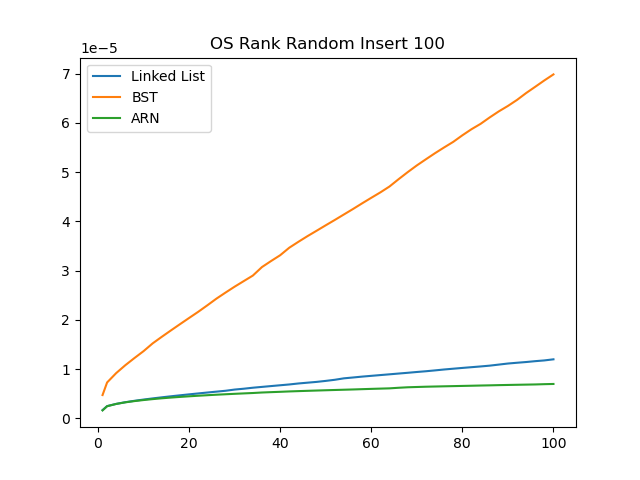
\includegraphics[width=0.8\linewidth]{Images/100/OS Rank Random Insert 100.png}
  \caption{OS Rank Random Insert 100}
  \label{fig:OS Rank Random Insert 100}
  \end{figure}
  \begin{figure}[H]
  \centering
  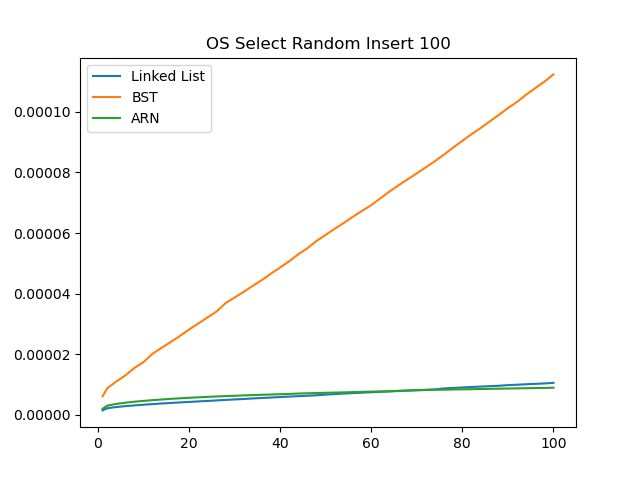
\includegraphics[width=0.8\linewidth]{Images/100/OS Select Random Insert 100.png}
  \caption{OS Select Random Insert 100}
  \label{fig:OS Select Random Insert 100}
\end{figure}
 \begin{figure}[H]
  \centering
  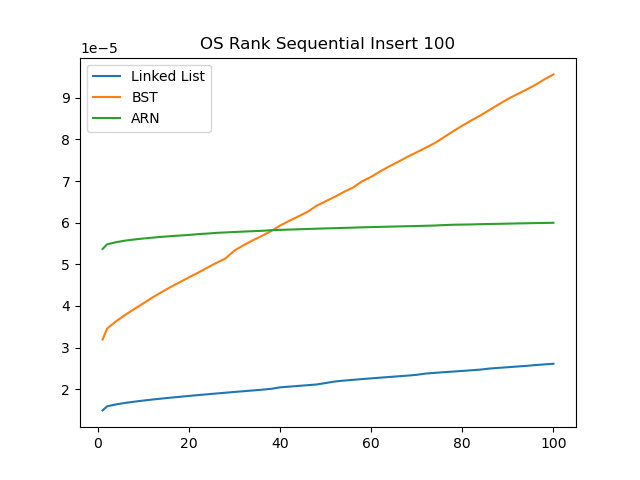
\includegraphics[width=0.8\linewidth]{Images/100/OS Rank Sequential Insert 100.png}
  \caption{OS Rank Sequential Insert 100 }
  \label{fig:OS Rank Sequential Insert 100}
\end{figure}
 \begin{figure}[H]
  \centering
  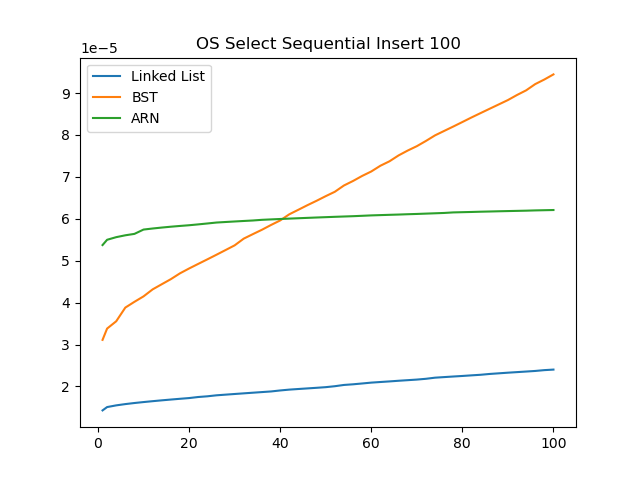
\includegraphics[width=0.8\linewidth]{Images/100/OS Select Sequential Insert 100.png}
  \caption{OS Select Sequential Insert 100 }
  \label{fig:OS Select Sequential Insert 500}
\end{figure}
 \begin{figure}[H]
  \centering
  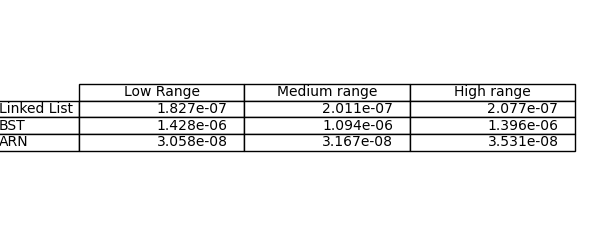
\includegraphics[width=0.8\linewidth]{Images/100/OS Rank Random Insert 100 Table.png}
  \caption{OS Rank Random Insert 100 Table }
  \label{fig:OS Rank Random Insert 100 Table}
\end{figure}
 \begin{figure}[H]
  \centering
  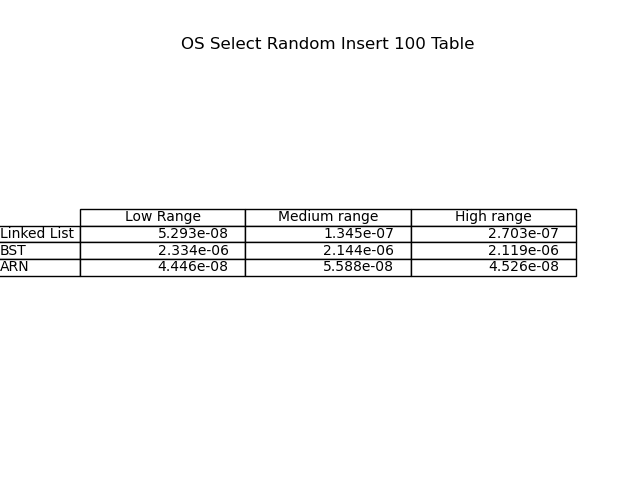
\includegraphics[width=0.8\linewidth]{Images/100/OS Select Random Insert 100 Table.png}
  \caption{OS Select Random Insert 100 Table }
  \label{fig:OS Select Random Insert 100 Table}
\end{figure}
 \begin{figure}[H]
  \centering
  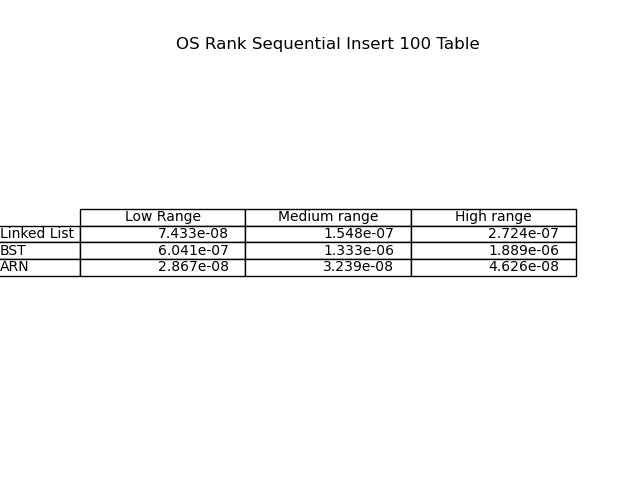
\includegraphics[width=0.8\linewidth]{Images/100/OS Rank Sequential Insert 100 Table.png}
  \caption{OS Rank Sequential Insert 100 Table }
  \label{fig:OS Rank Sequential Insert 100 Table}
\end{figure}
 \begin{figure}[H]
  \centering
  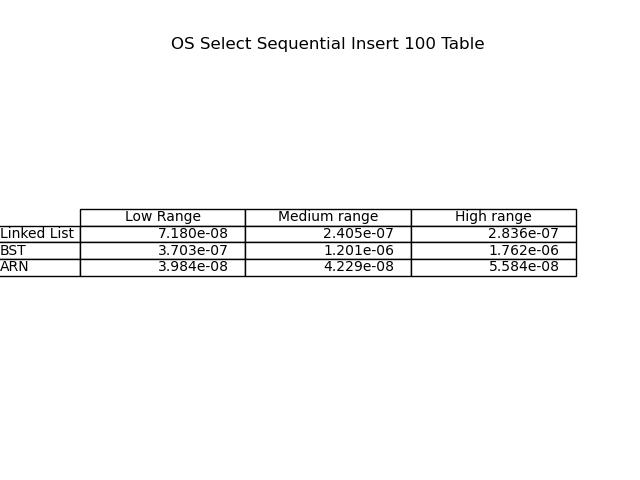
\includegraphics[width=0.8\linewidth]{Images/100/OS Select Sequential Insert 100 Table.png}
  \caption{OS Select Sequential Insert 100 Table }
  \label{fig:OS Select Sequential Insert 100 Table}
\end{figure}
\subsubsection{500 elements}

In this case, we will choose $K = 100$. 
Figures
\ref{fig:OS Rank Random Insert 500} - \ref{fig:OS Select Sequential Insert 500} confirm the hypotheses formulated in the previous case regarding the linear behavior (for lists and ABR) and logarithmic behavior (for ARN). However, it can be observed that for larger data structures, the implementation on ARN is faster compared to that on ordered lists, while the gap with the approach that uses BST starts to widen increasingly.

 \begin{figure}[H]
  \centering
  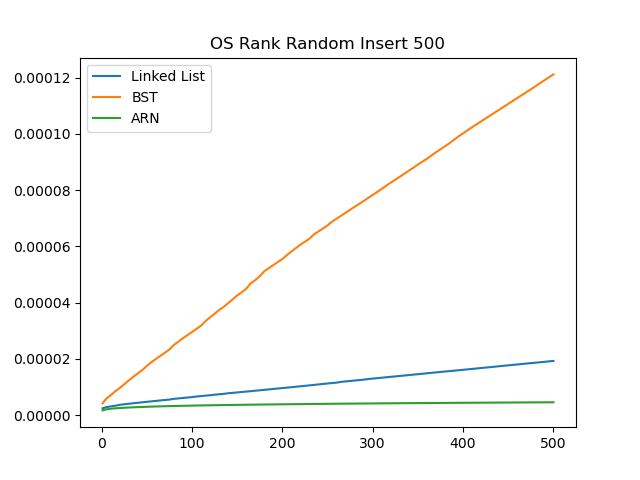
\includegraphics[width=0.8\linewidth]{Images/500/OS Rank Random Insert 500.png}
  \caption{OS Rank Random Insert 500 }
  \label{fig:OS Rank Random Insert 500}
\end{figure}
 \begin{figure}[H]
  \centering
  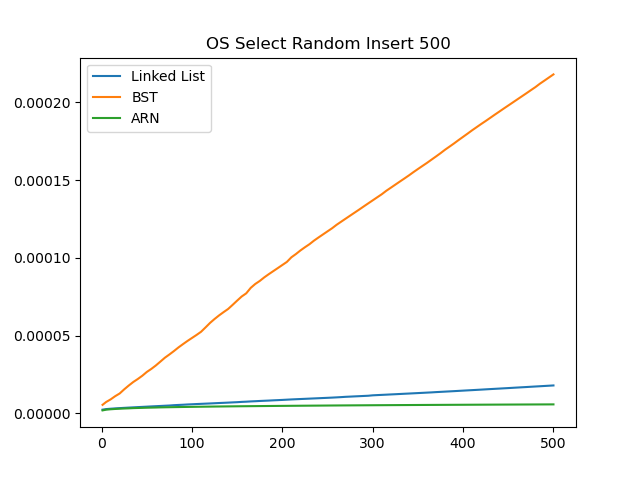
\includegraphics[width=0.8\linewidth]{Images/500/OS Select Random Insert 500.png}
  \caption{OS Select Random Insert 500 }
  \label{fig:OS Select Random Insert 500}
\end{figure}
 \begin{figure}[H]
  \centering
  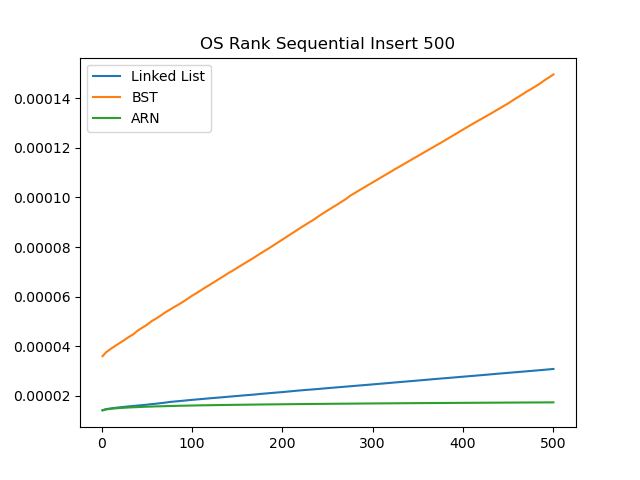
\includegraphics[width=0.8\linewidth]{Images/500/OS Rank Sequential Insert 500.png}
  \caption{OS Rank Sequential Insert 500 }
  \label{fig:OS Rank Sequential Insert 500}
\end{figure}
 \begin{figure}[H]
  \centering
  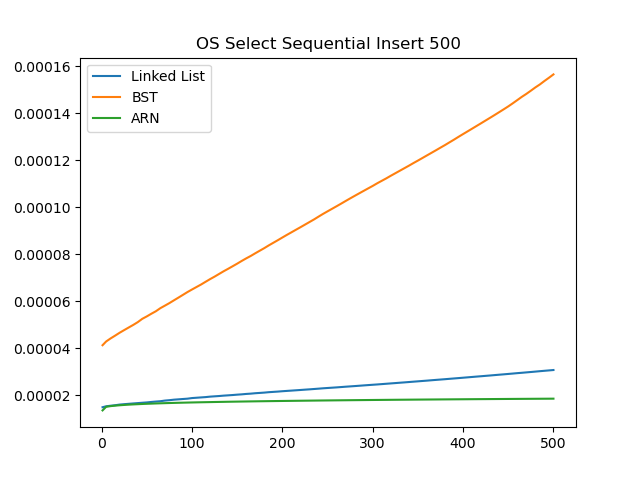
\includegraphics[width=0.8\linewidth]{Images/500/OS Select Sequential Insert 500.png}
  \caption{OS Select Sequential Insert 500 }
  \label{fig:OS Select Sequential Insert 500}
\end{figure}
 \begin{figure}[H]
  \centering
  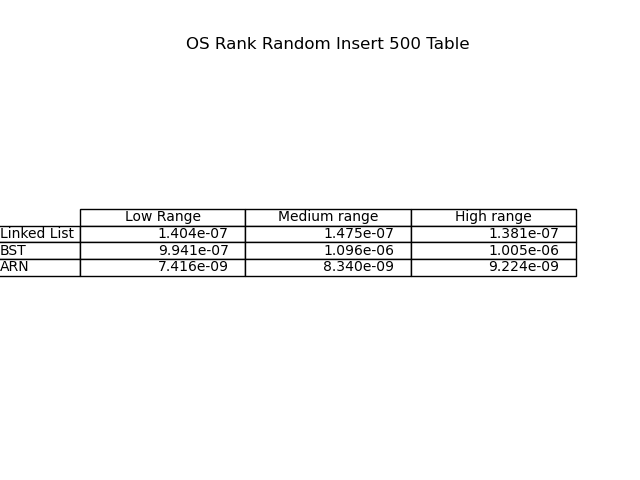
\includegraphics[width=0.8\linewidth]{Images/500/OS Rank Random Insert 500 Table.png}
  \caption{OS Rank Random Insert 500 Table }
  \label{fig:OS Rank Random Insert 500 Table}
\end{figure}
 \begin{figure}[H]
  \centering
  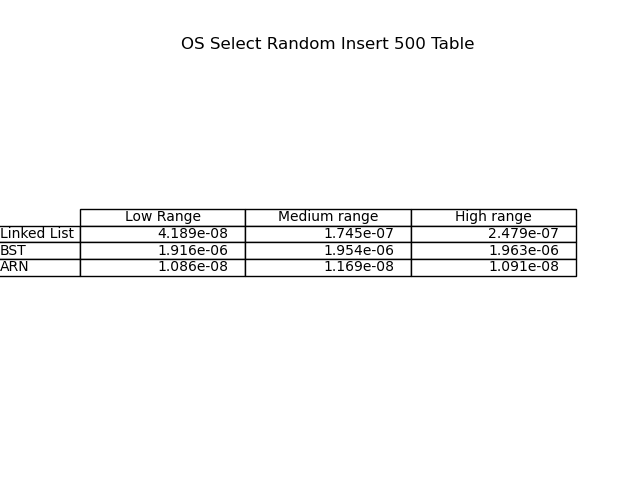
\includegraphics[width=0.8\linewidth]{Images/500/OS Select Random Insert 500 Table.png}
  \caption{OS Select Random Insert 500 Table }
  \label{fig:OS Select Random Insert 500 Table}
\end{figure}
 \begin{figure}[H]
  \centering
  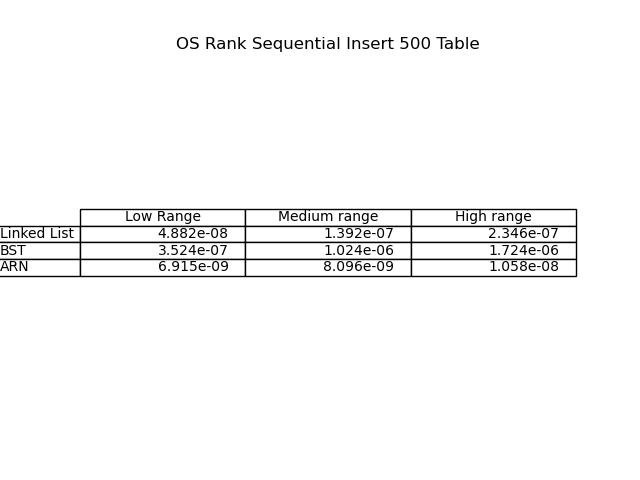
\includegraphics[width=0.8\linewidth]{Images/500/OS Rank Sequential Insert 500 Table.png}
  \caption{OS Rank Sequential Insert 500 Table }
  \label{fig:OS Rank Sequential Insert 500 Table}
\end{figure}
 \begin{figure}[H]
  \centering
  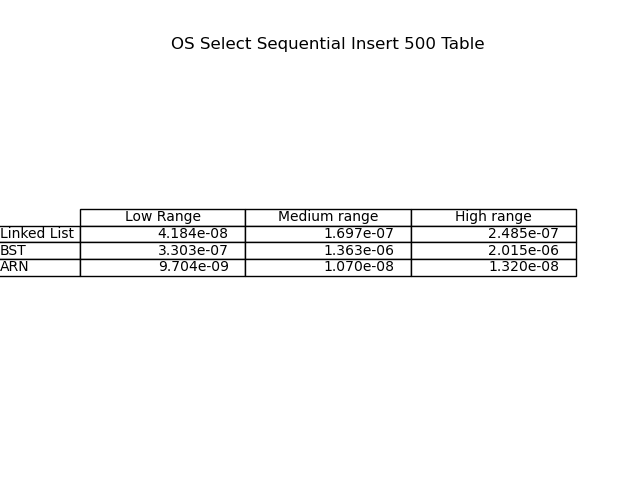
\includegraphics[width=0.8\linewidth]{Images/500/OS Select Sequential Insert 500 Table.png}
  \caption{OS Select Sequential Insert 500 Table }
  \label{fig:OS Select Sequential Insert 500 Table}
\end{figure}
\subsubsection{1000 elements}

In this case, we'll also choose $K = 100$. Having verified in previous cases the complexity of the different implementations of the OS algorithms, in this instance, we'll only comment on the graphs that allow us to compare them. By observing Figures \ref{fig:OS Rank Random Insert 1000}-\ref{fig:OS Select Sequential Insert 1000}, it can be noted that for large data structures, the OS algorithms perform much better in the case of ARNs with the 'size' attribute, while the gap in terms of execution time between the implementation on BST and those on other data structures is even more evident.

Now, let's analyze the average execution times for the three ranges of indices/nodes entering the OS Select and OS Rank functions, as observable in Figures \ref{fig:OS Rank Random Insert 1000 Table}-\ref{fig:OS Select Sequential Insert 1000 Table}. We immediately notice that the performances in the case of ARNs are similar in all three ranges, and this situation doesn't change even if the data insertion is randomized, since the insertFixup() function precisely maintains the tree balanced with each new insertion. 

In the case of ordered lists, on the other hand, we notice how the algorithms are faster in the lower range and slower in the higher one; this is because the indices/nodes are searched starting from the first ones. Few differences, instead, in the case of random insertion, since, being the list ordered, the order of the nodes in the list is not influenced by their insertion order.

As for BSTs with sequential insertion, we can make a similar argument to the one made for lists, since the implementations of the OS algorithms on these data structures are based on the same underlying idea (we can also think that a completely unbalanced binary tree becomes a list). In the case of random insertion, however, we find ourselves with a definitely more balanced tree, and this is also reflected in the performances, which, as in the case of ARN, are now more balanced.
 \begin{figure}[H]
  \centering
  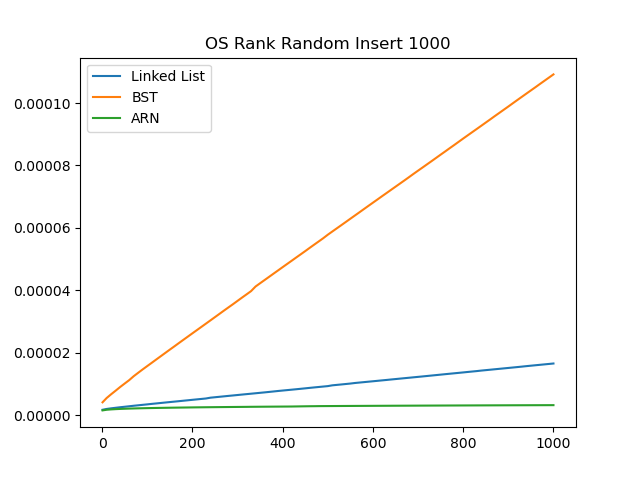
\includegraphics[width=0.8\linewidth]{Images/1000/OS Rank Random Insert 1000.png}
  \caption{OS Rank Random Insert 1000 }
  \label{fig:OS Rank Random Insert 1000}
\end{figure}
 \begin{figure}[H]
  \centering
  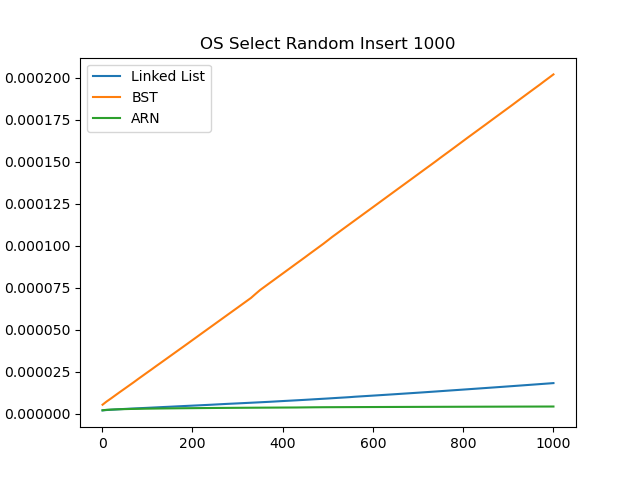
\includegraphics[width=0.8\linewidth]{Images/1000/OS Select Random Insert 1000.png}
  \caption{OS Select Random Insert 1000 }
  \label{fig:OS Select Random Insert 1000}
\end{figure}
 \begin{figure}[H]
  \centering
  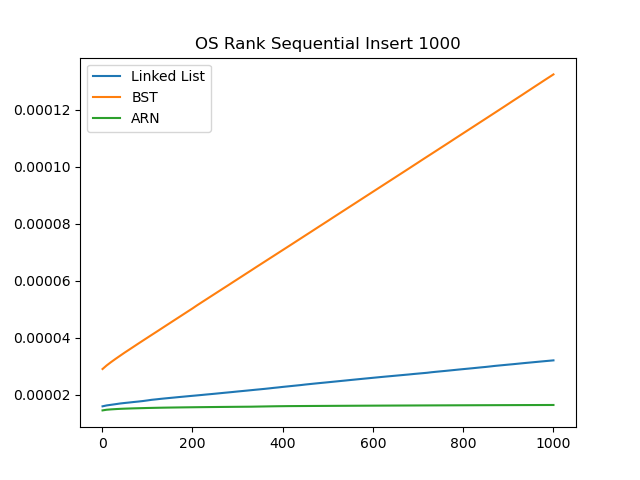
\includegraphics[width=0.8\linewidth]{Images/1000/OS Rank Sequential Insert 1000.png}
  \caption{OS Rank Sequential Insert 1000 }
  \label{fig:OS Rank Sequential Insert 1000}
\end{figure}
 \begin{figure}[H]
  \centering
  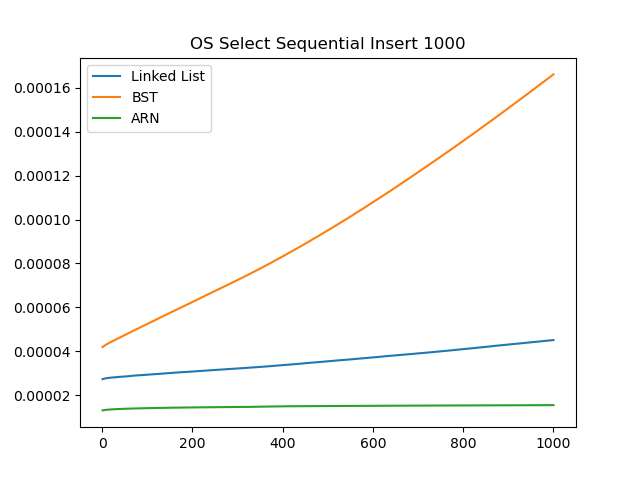
\includegraphics[width=0.8\linewidth]{Images/1000/OS Select Sequential Insert 1000.png}
  \caption{OS Select Sequential Insert 1000 }
  \label{fig:OS Select Sequential Insert 1000}
\end{figure}
 \begin{figure}[H]
  \centering
  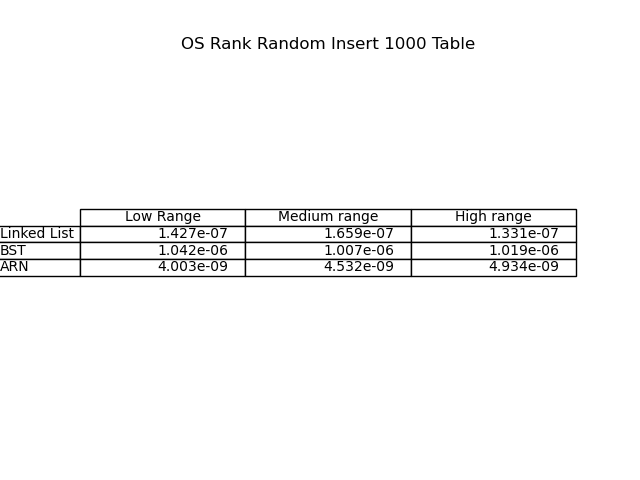
\includegraphics[width=0.8\linewidth]{Images/1000/OS Rank Random Insert 1000 Table.png}
  \caption{OS Rank Random Insert 1000 Table }
  \label{fig:OS Rank Random Insert 1000 Table}
\end{figure}
 \begin{figure}[H]
  \centering
  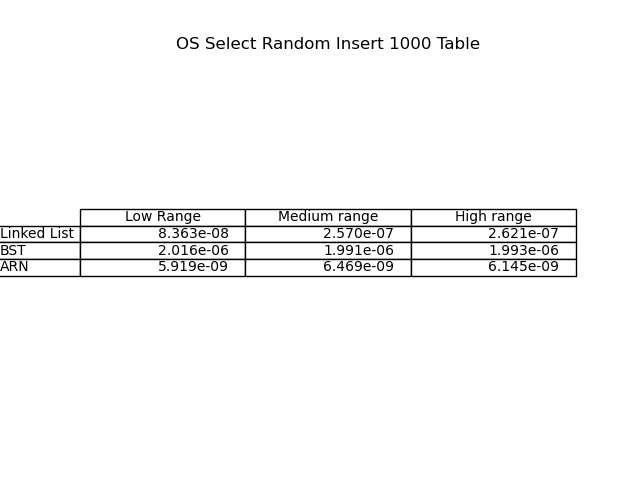
\includegraphics[width=0.8\linewidth]{Images/1000/OS Select Random Insert 1000 Table.png}
  \caption{OS Select Random Insert 1000 Table }
  \label{fig:OS Select Random Insert 1000 Table}
\end{figure}
 \begin{figure}[H]
  \centering
  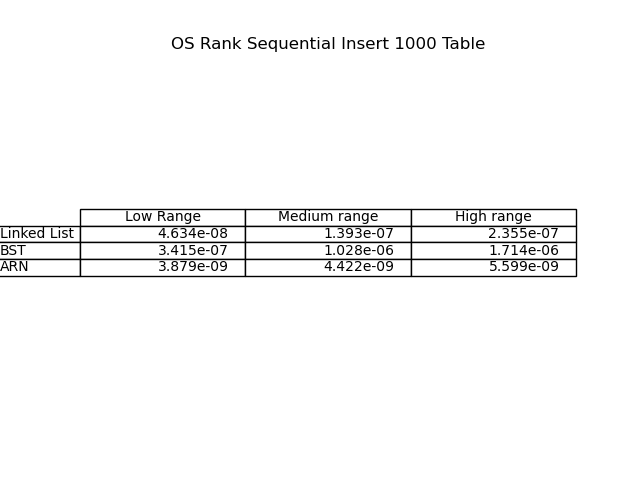
\includegraphics[width=0.8\linewidth]{Images/1000/OS Rank Sequential Insert 1000 Table.png}
  \caption{OS Rank Sequential Insert 1000 Table }
  \label{fig:OS Rank Sequential Insert 1000 Table}
\end{figure}
 \begin{figure}[H]
  \centering
  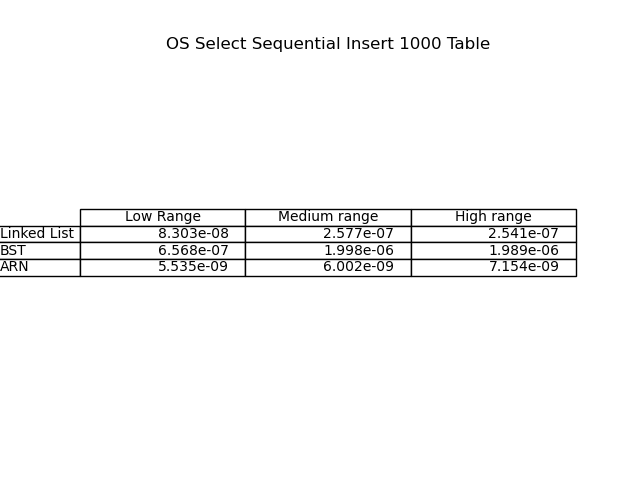
\includegraphics[width=0.8\linewidth]{Images/1000/OS Select Sequential Insert 1000 Table.png}
  \caption{OS Select Sequential Insert 1000 Table }
  \label{fig:OS Select Sequential Insert 1000 Table}
\end{figure}
\subsubsection{1500 elements}
For this final test, it was necessary to allocate more memory to VisualStudio to handle the high number of recursive calls.

In this case as well, we will only observe the graphs that compare the performances on different data structures (Figures 18 and 19), printed by choosing $K = 300$.

These last tests only confirm the observations made in previous cases, showing how the implementation on BST becomes less performant as the input sizes increase, while the implementation on ARN maintains satisfactory execution times even in the face of much larger data structures.
 \begin{figure}[H]
  \centering
  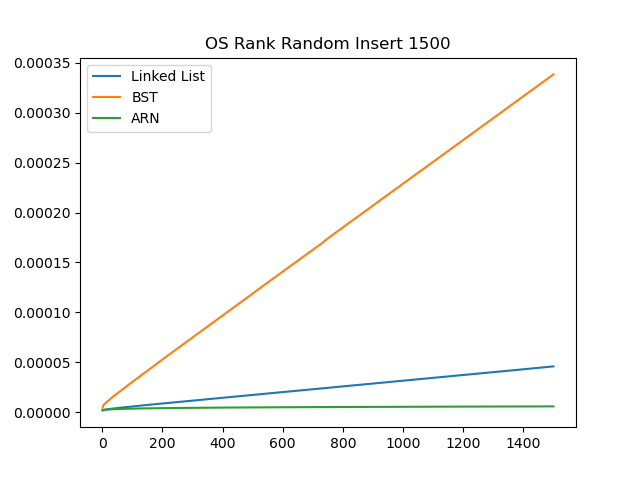
\includegraphics[width=0.8\linewidth]{Images/1500/OS Rank Random Insert 1500.png}
  \caption{OS Rank Random Insert 1500 }
  \label{fig:OS Rank Random Insert 1500}
\end{figure}
 \begin{figure}[H]
  \centering
  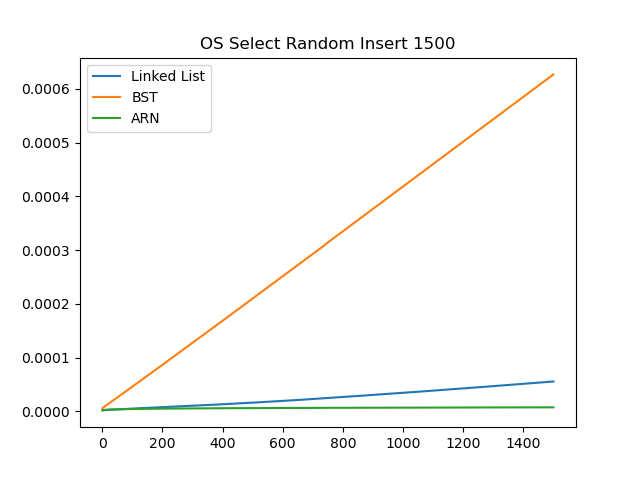
\includegraphics[width=0.8\linewidth]{Images/1500/OS Select Random Insert 1500.png}
  \caption{OS Select Random Insert 1500 }
  \label{fig:OS Select Random Insert 1500}
\end{figure}
 \begin{figure}[H]
  \centering
  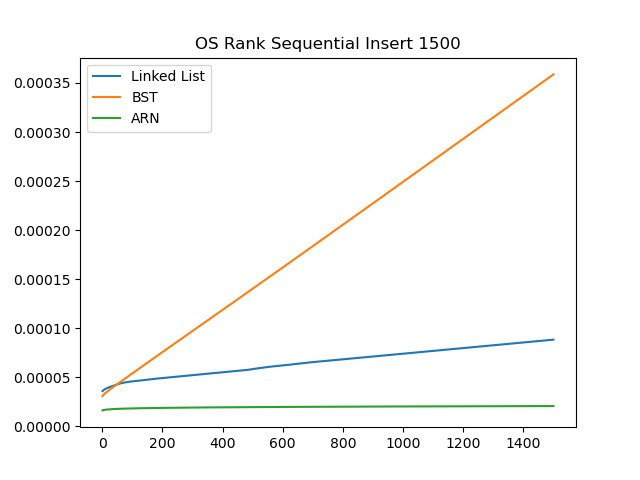
\includegraphics[width=0.8\linewidth]{Images/1500/OS Rank Sequential Insert 1500.png}
  \caption{OS Rank Sequential Insert 1500 }
  \label{fig:OS Rank Sequential Insert 1500}
\end{figure}
 \begin{figure}[H]
  \centering
  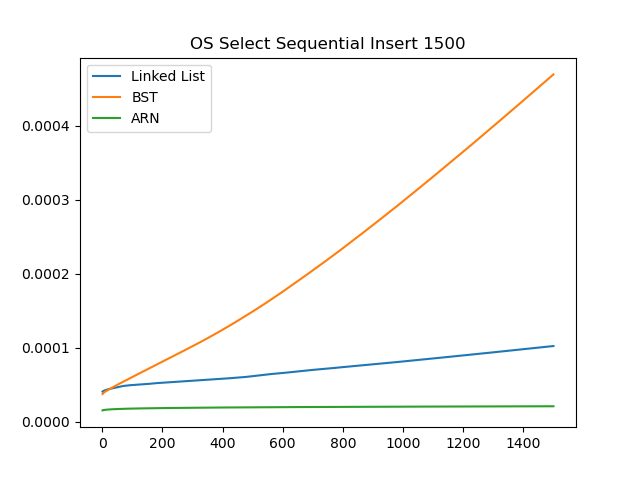
\includegraphics[width=0.8\linewidth]{Images/1500/OS Select Sequential Insert 1500.png}
  \caption{OS Select Sequential Insert 1500 }
  \label{fig:OS Select Sequential Insert 1500}
\end{figure}
 \begin{figure}[H]
  \centering
  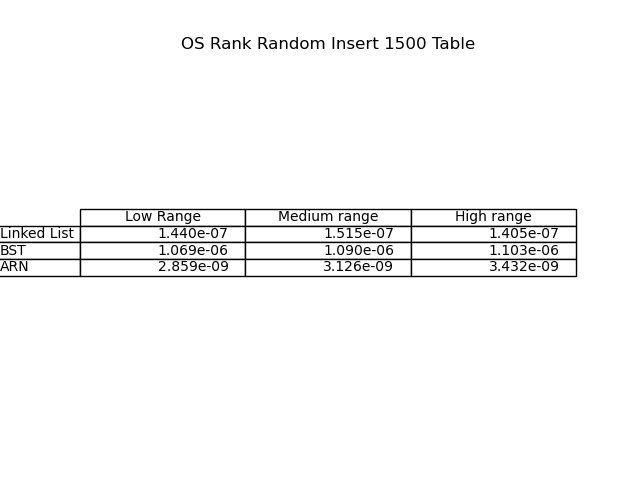
\includegraphics[width=0.8\linewidth]{Images/1500/OS Rank Random Insert 1500 Table.png}
  \caption{OS Rank Random Insert 1500 Table }
  \label{fig:OS Rank Random Insert 1500 Table}
\end{figure}
 \begin{figure}[H]
  \centering
  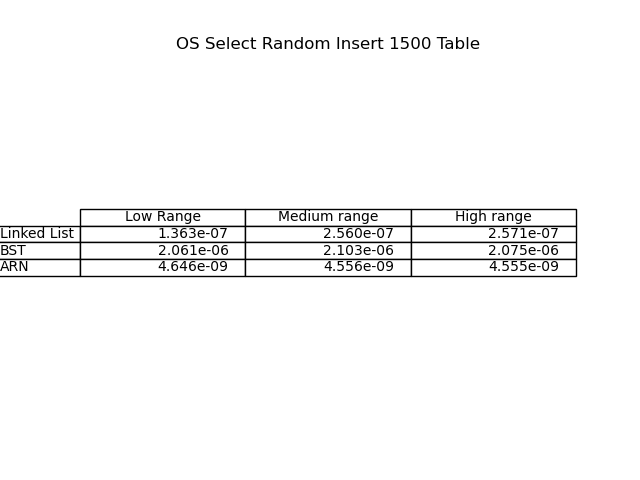
\includegraphics[width=0.8\linewidth]{Images/1500/OS Select Random Insert 1500 Table.png}
  \caption{OS Select Random Insert 1500 Table }
  \label{fig:OS Select Random Insert 1500 Table}
\end{figure}
 \begin{figure}[H]
  \centering
  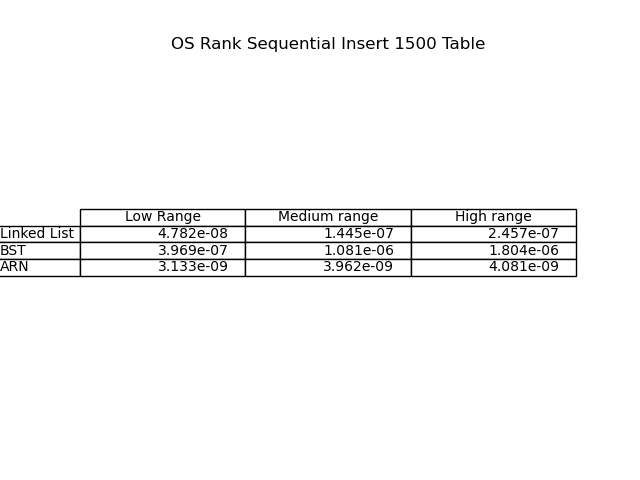
\includegraphics[width=0.8\linewidth]{Images/1500/OS Rank Sequential Insert 1500 Table.png}
  \caption{OS Rank Sequential Insert 1500 Table }
  \label{fig:OS Rank Sequential Insert 1500 Table}
\end{figure}
 \begin{figure}[H]
  \centering
  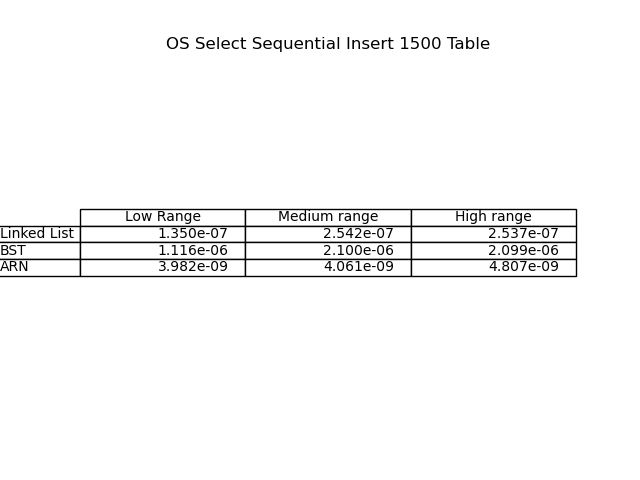
\includegraphics[width=0.8\linewidth]{Images/1500/OS Select Sequential Insert 1500 Table.png}
  \caption{OS Select Sequential Insert 1500 Table }
  \label{fig:OS Select Sequential Insert 1500 Table}
\end{figure}
\section{Test discussion and conclusions}
The results of the tests conducted confirm the hypotheses made previously regarding the complexity of the OS algorithms in the different implementations: we are talking about $O(n)$ for ordered lists and search trees and $O(lg(n))$ for ARNs, regardless of the type of insertion adopted.

The implementation for ARNs with the size attribute proves to be the most performant in general and reports similar performances regardless of the requested node/index.

Ordered lists, on the other hand, are a valid choice for data structures of small sizes, particularly fast when dealing with the first elements of the list.

Finally, the implementation for BSTs without the size attribute has proven to be the least effective, as the absence of this parameter makes it impossible to exploit the potential of the data structure and instead forces a much less elaborate approach similar to that adopted for lists. The performances on BSTs are much worse due to the time spent descending and ascending the tree through recursive calls, and even when the tree is more balanced, the improvement in terms of performance is relative.
\end{document}
